%%%%%%%%%%%%%%%%%%%%%%%%%%%%%%%%%%%%%%%%%%%%%%%%%%%%%%%%%%%%%%%%%%%%%%%%
%     LaTeX source code to approximate a Draft NIST Technical report
%	  Instructions for authors: tinyurl.com/techpubsnist 
%	DOI watermark will be added on final PDF
% 	Developed by K. Miller, kmm5@nist.gov 
%	Last updated: 22-March-2019
%%%%%%%%%%%%%%%%%%%%%%%%%%%%%%%%%%%%%%%%%%%%%%%%%%%%%%%%%%%%%%%%%%%

%%%%%%%%%%%%%%%%%%%%%%
% Template further altered by Armen Amirkhanian
% for use with UA lab courses in an effort to 
% have a standardized format for lab documents
% Last update 9-April-2020
%
% TODO:
% --Get the appendices to dynamically link, tocloft causes problems
%%%%%%%%%%%%%%%%%%%%%%

\documentclass[12pt]{article}
\usepackage{amsmath}
\usepackage{amsfonts}   % if you want the fonts
\usepackage{amssymb}    % if you want extra symbols
\usepackage{graphicx}   % need for figures
\usepackage{xcolor}
\usepackage{bm}
\usepackage{secdot}		
\usepackage{mathptmx}
\usepackage{float}
\usepackage[utf8]{inputenc}
\usepackage{textcomp}
\usepackage[hang,flushmargin,bottom]{footmisc} % footnote format
\usepackage{xspace}
%\usepackage{lineno}
\usepackage{ragged2e}
\usepackage{parskip}
\usepackage{textcomp}

\usepackage{tikz}
\usetikzlibrary{shapes.geometric, arrows}
\tikzstyle{startstop} = [rectangle, rounded corners, minimum width=2cm, minimum height=1cm,text centered, draw=black, fill=red!20]
\tikzstyle{arrow} = [thick,->,>=stealth]

\usepackage{titlesec}
\titleformat{\section}{\normalsize\bfseries}{\thesection.}{1em}{}	% required for heading numbering style
\titleformat*{\subsection}{\normalsize\bfseries}

\usepackage{tocloft}	% change typeset, titles, and format list of appendices/figures/tables
\renewcommand{\cftdot}{}	
\renewcommand{\contentsname}{Table of Contents}
\renewcommand{\cftpartleader}{\cftdotfill{\cftdotsep}} % for parts
\renewcommand{\cftsecleader}{\cftdotfill{\cftdotsep}}
\renewcommand\cftbeforesecskip{\setlength{4pt}{}}
\addtolength{\cftfignumwidth}{1em}
\renewcommand{\cftfigpresnum}{\figurename\ }
\addtolength{\cfttabnumwidth}{1em}
\renewcommand{\cfttabpresnum}{\tablename\ }
\setlength{\cfttabindent}{0in}    %% adjust as you like
\setlength{\cftfigindent}{0in} 

\usepackage{enumitem}         % to control spacing between bullets/numbered lists

\usepackage[numbers,sort&compress]{natbib} % format bibliography 
\renewcommand{\bibsection}{}
\setlength{\bibsep}{0.0pt}

\usepackage[hidelinks]{hyperref}
\hypersetup{
	colorlinks = true,
urlcolor ={blue},
citecolor = {.},
linkcolor = {.},
anchorcolor = {.},
filecolor = {.},
menucolor = {.},
runcolor = {.}
pdftitle={},
pdfsubject={},
pdfauthor={},
pdfkeywords={}
}
\urlstyle{same}

\usepackage{epstopdf} % converting EPS figure files to PDF

\usepackage{fancyhdr, lastpage}	% formatting document, calculating number of pages, formatting headers
\setlength{\topmargin}{-0.5in}
\setlength{\headheight}{39pt}
\setlength{\oddsidemargin}{0.25in}
\setlength{\evensidemargin}{0.25in}
\setlength{\textwidth}{6.0in}
\setlength{\textheight}{8.5in}

\usepackage{caption} % required for Figure labels
\captionsetup{font=small,labelfont=bf,figurename=Fig.,labelsep=period,justification=raggedright} 

%%%%%%%%%%% !!!!!REQUIRED - FILL OUT METADATA HERE !!!!!!!! %%%%%%%%%%%%%%
%%%%%%%%%%%%%%%%%%%%%%%%%%%%%%%%%%%%%%%%%%%%%%%%%%%%%%%%%%%%%%%%%%%%%%%%%%
\newcommand{\CourseNum}{CE340}
\newcommand{\CourseName}{Geotechnical Engineering}
\newcommand{\LabTitle}{Standard Proctor}
\newcommand{\LastUpdate}{Summer 2020}

%%%%%%%%%%%%%%%%%%%%%%%%%%%%%%%%%%%%%%%%%%%%%%%%%%%%%%%%%%%%%%%%%%%%
%   	BEGIN DOCUMENT 
%%%%%%%%%%%%%%%%%%%%%%%%%%%%%%%%%%%%%%%%%%%%%%%%%%%%%%%%%%%%%%%%%%%%
\begin{document}
	\urlstyle{rm} % Format style of \url   
%\linenumbers
\begin{titlepage}
\begin{flushright}
\LARGE{\textbf{\CourseNum{} -- \CourseName}}\\
\vfill
\Huge{\textbf{\LabTitle}}\\
    \vfill
%%%%%%%%%%%%%%%%%%%%%%%%%%%%%%%%%%%%%%%%%%%%%%%%%%%%%%%%%%%%%%%%%%%%
%	Authors - add complete list of authors, affiliations will be 
%   added on title page
%%%%%%%%%%%%%%%%%%%%%%%%%%%%%%%%%%%%%%%%%%%%%%%%%%%%%%%%%%%%%%%%%%%%
    \large Dr. Armen Amirkhanian, P.E.\\
    \normalsize Sam Prather (Reviewer)\\
\vfill
%%%%%%%%%%%%%%%%%%%%%%%%%%%%%%%%%%%%%%%%%%%%%%%%%%%%%%%%%%%%%%%%%%%%
%	The DOI is automated based on metadata.	
%%%%%%%%%%%%%%%%%%%%%%%%%%%%%%%%%%%%%%%%%%%%%%%%%%%%%%%%%%%%%%%%%%%%
\normalsize This work is licensed under the Creative Commons Attribution-ShareAlike 4.0 International License. To view a copy of this license, visit:
\href{http://creativecommons.org/licenses/by-sa/4.0/}{http://creativecommons.org/licenses/by-sa/4.0/}.

\includegraphics[width=0.07\textwidth]{cc.eps}
\includegraphics[width=0.07\textwidth]{by.eps}
\includegraphics[width=0.07\textwidth]{sa.eps}
\vfill

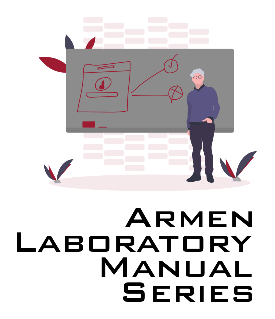
\includegraphics[width=0.3\linewidth]{Logo.eps}\\ 
 
  
\end{flushright}
\end{titlepage}

\begin{titlepage}
\begin{center}
\normalsize 
Certain commercial entities, equipment, or materials may be identified in this document in order to describe an experimental procedure or concept adequately. Such identification is not intended to imply recommendation or endorsement by The University of Alabama or the listed authors, nor is it intended to imply that the entities, materials, or equipment are necessarily the best available for the purpose.\\

\vfill
Any opinions or recommendations are solely those of the authors and do not represent the official view or policy of The University of Alabama.
\end{center}
\begin{flushright}
\vfill
\normalsize 
This document was last updated in \textbf{\LastUpdate} and should contain \textbf{\pageref{LastPage}} pages of content exclusive of these title pages, abstract, and other front matter. If the document appears to be incomplete, please contact the author(s).\\
\vfill
It is not unscientific to make a guess,\\although many people who are not in science think it is.\\
\textit{Richard Feynman}
\end{flushright}
\end{titlepage}
%%%%%%%%%%%%%%%%%%%%%%%%%%%%%%%%%%%%%%%%%%%%%%%%%%%%%%%%%%%%%%%%%%%%
%   Start front matter - page number starts with "i"
%%%%%%%%%%%%%%%%%%%%%%%%%%%%%%%%%%%%%%%%%%%%%%%%%%%%%%%%%%%%%%%%%%%%
\pagenumbering{roman}
\section*{Abstract}
\normalsize Compaction of soils is an important part of many civil engineering projects. It is not usually sufficient to compact a soil to a point at which it looks good. We need to understand how compacted our soil can be so that we can perform design calculations. Additionally, we need to know the maximum possible compaction we can achieve with a soil so that we can check compaction in the field during the construction process. The most common method to evaluate the compactability of a soil is called the Proctor method, named after R.R. Proctor who developed the method in 1933. The testing procedure involves compacting a series of soil samples at increasing moisture contents. The resulting data is plotted and the maximum unit weight can be determined. Associated with this parameter is the optimum moisture content.\\

\vfill
\section*{Keywords}
\normalsize compaction; proctor test; moisture-density curve; optimum moisture content; maximum dry density.\\
\pagebreak
%%%%%%%%%%%%%%%%%%%%%%%%%%%%%%%%%%%%%%%%%%%%%%%%%%%%%%%%%%%%%%%%%%%%
%   Table of Contents is required
% 	List of Tables & Figures required if more than 5 tables/figures
%%%%%%%%%%%%%%%%%%%%%%%%%%%%%%%%%%%%%%%%%%%%%%%%%%%%%%%%%%%%%%%%%%%%
\begin{center}
\tableofcontents
\pagebreak
\listoftables
\listoffigures
\end{center}
\pagebreak
\section*{Required Specifications}
The following specifications are required to complete this laboratory exercise:
\begin{description}
\item[ASTM D698] Standard Test Methods for Laboratory Compaction Characteristics of Soil Using Standard Effort (12,400 ft-lbf/ft$^3$ (600 kN-m/m$^3$))
\end{description}

The following specifications are optional, but they are listed here in the event more information is needed to complete the laboratory exercise:
\begin{description}
\item[ASTM D6026] Standard Practice for Using Significant Digits in Geotechnical Data
\item[ASTM E11] Specification for Woven Wire Test Sieve Cloth and Test Sieves
\end{description}
\pagebreak
%%%%%%%%%%%%%%%%%%%%%%%%%%%%%%%%%%%%%%%%%%%%%%%%%%%%%%%%%%%%%%%%%%%%
%   Start body of text - page number starts with "1"
%%%%%%%%%%%%%%%%%%%%%%%%%%%%%%%%%%%%%%%%%%%%%%%%%%%%%%%%%%%%%%%%%%%%
\section{Compaction}
\label{sec:intro}
\pagenumbering{arabic}
\normalsize 
The standard Proctor test has been around for nearly 80 years. It is a reliable workhorse test method that provides valuable data for design and construction. A known weight is repeatedly dropped from a constant height to compact a soil specimen in a cylindrical mold. The mass and volume are determined and the resulting unit weight can be calculated. This is done for a series of moisture contents to establish what is called the moisture-density curve.

The standard Proctor test, ASTM D698, simulates the compaction achieved with relatively small compaction equipment, such as hand tampers, vibratory walk-behind compactors, jumping jacks, etc. Modern virbatory roller compactors can put significant compactive effort into the soil. There is a modified Proctor test, ASTM D1557, which better simulates the compaction seen when using large compaction equipment. The primary difference between the two methods is the weight and height of the drop for the compaction. The remainder of the procedure is nearly identical.

\subsection{Objectives}
\label{ssec:headingscap}
At the completion of this lab exercise, you will have satisfied the following objectives:
\begin{enumerate}
    \item Perform a series of compaction tests using the standard Proctor method
    \item Perform calculations necessary to create a moisture-density curve
\end{enumerate}

\subsection{Learning Outcomes}
At the completion of this lab exercise, you should be able to:
\begin{itemize}
    \item understand what the laboratory compaction process represents
    \item perform calculations necessary to determine the maximum dry unit weight and optimum moisture content of a soil sample
    \item understand how to interpret information from a moisture-density curve
\end{itemize}

\pagebreak
\subsection{Procedure}
The standard Proctor test procedure is divided into three parts: preparation, execution, and analysis. While the test can be run on moist and dry samples, it is preferred that the test be run on moist samples (ASTM D698 \S10.2). Additionally, samples should not be reused for further compaction per ASTM D698 \S10.1.1. You will be provided with sufficient moist material that you will be able to run three compaction tests without needing to reuse the soil.

\subsubsection{Preparation}
You will need three pieces of equipment for this procedure: compaction hammer, compaction mold, three sample containers, and a scale. For the standard Proctor method, the hammer is 5.5 lbs. Since the soil is relatively fine, a 4-inch diameter mold is appropriate.

You will need to determine the empty weight of the compaction mold. While we can remove the sample from the mold most of the time, we sometimes lose too much material. We will obtain the weight of the compacted soil while still in the mold and will need to subtract the weight of the mold from the measurement. You will be provided with the volume of the mold for use in calculations during the analysis portion.

\subsubsection*{Preparation Checklist}
\begin{itemize}
    \item Obtain compaction hammer and compaction mold
    \item Obtain empty weight of compaction mold
    \item Obtain the weights of the three sample containers
\end{itemize}

\subsubsection{Execution}
The execution process is straightforward. You will compact the soil in the mold using three layers of equal height. Each layer is compacted with 25 drops of the hammer. It takes some experience to know how much soil to add for each layer, especially the first layer, so that you end up with three equal layers. It is important to begin the compaction of each layer properly in terms of the pattern (Fig. \ref{fig:compactionpattern}). The four quadrants will first be compacted followed by a blows that go in a circular pattern around the mold until a total count of 25 blows has been achieved.

\begin{figure}
    \centering
    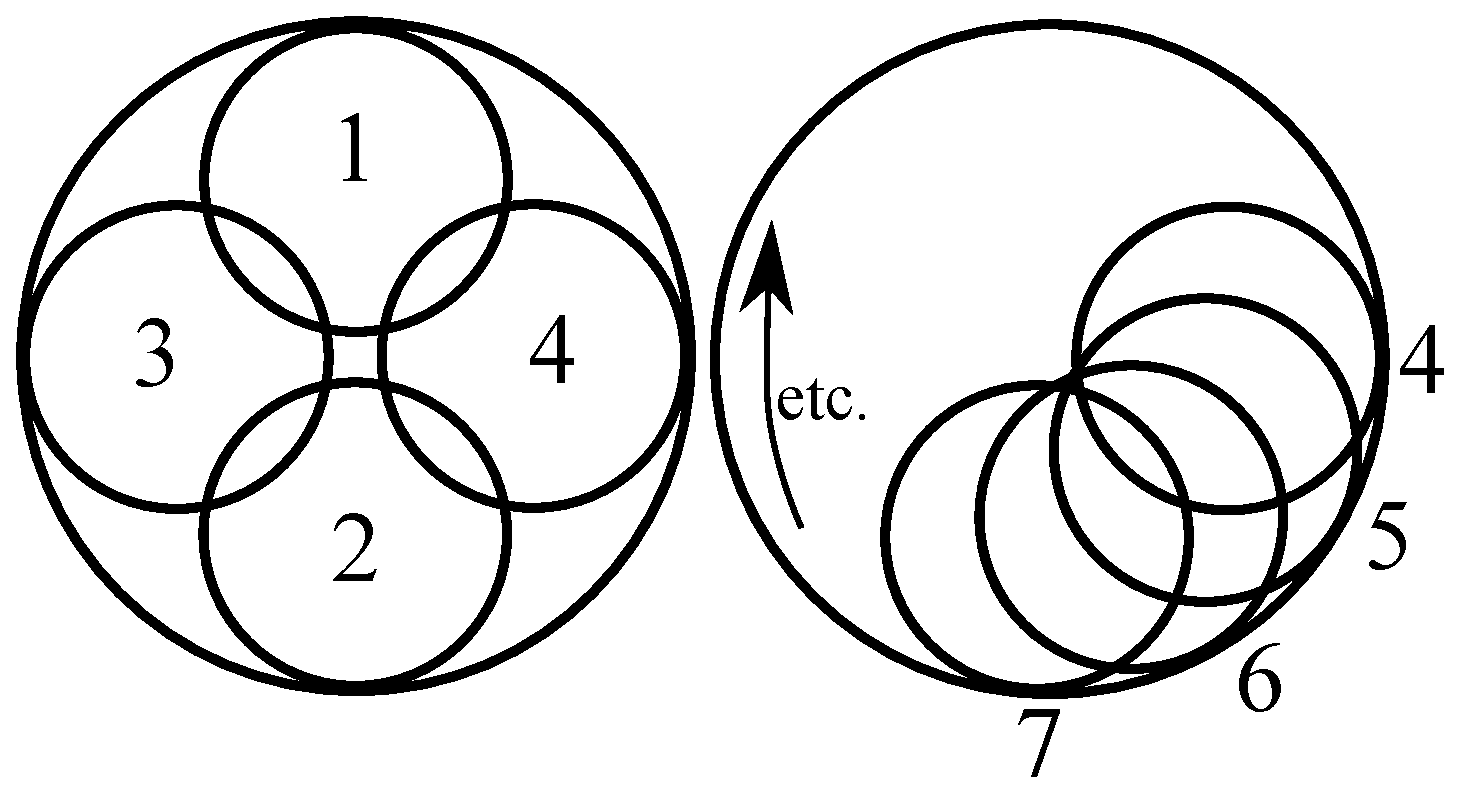
\includegraphics[width=0.8\textwidth]{compactionpattern.eps}
    \caption{Schematic of compaction pattern required in ASTM D698. The four quadrants are first compacted with one blow each followed by circular compaction around the perimeter of the circle.}
    \label{fig:compactionpattern}
\end{figure}

Occasionally, an uneven surface may develop during the compaction process. While the pattern is explicitly stated in ASTM D698, there is a provision in \S10.4.5 to allow the operator to exercise professional judgement to ensure the specimen is compacted evenly. It is important that each layer be relatively even, especially the top layer. ASTM D698 \S10.4.3 states that the final compacted layer height can exceed the top of the mold by a maximum of 0.25 inches or the entire test is discarded. Experience greatly increases the chance that the final height is within this tolerance.

After compaction of the top layer is complete, you will trim the excess height with a knife or similar straightedge. If there are any voids or ``potholes'' present in the top surface, you may fill those in with the remaining soil and use the straightedge to again strike off the top surface. Then you will obtain the weight of the compacted soil within the mold.

To determine the moisture content, we will take the compacted specimen out of the mold and oven dry it. Place as much as the sample as you can into the sample container weigh the moist soil sample. The specimen container will then be placed into a drying oven and you will be provided with the oven dry weights the next day. Ensure your specimen containers are properly labeled.

The next two compactions will be done in an identical manner except with additional water added to the soil specimens. For your second specimen, weigh out approximately 3 kg of moist soil. Then, calculate the amount of water you would need to add to your measured soil mass to increase the moisture content about 2\%. That is, if the moist soil starts at a moisture content of 5\%, how much water is needed to bring that moisture content to 7\%. Recall that the moisture content, $w$, is given by Eq. \ref{eq:MC}
\begin{equation}
    w=\dfrac{M_w}{M_s}=\dfrac{M_w}{M_t-M_w}
    \label{eq:MC}
\end{equation}
where $M_w$ is the mass of water, $M_s$ is the oven dry mass, and $M_t$ is the moist mass. However, we do not have the starting moisture content from the first compaction specimen yet. We need to exercise some engineering judgement. Estimate the moisture content of the starting sample! It is probably somewhere between 4\% and 7\%. So if we take our assumed moisture content, we can calculate the expected oven dry mass and then determine how much additional water is needed to increase the moisture content by 2\%.

For example, say we have 1 kg of a moist soil sample and we assume the moisture content to be 3\%. We want our next sample to be at 5\% so we need to determine how much additional water to add to go from 3\% to 5\%. From Eq. \ref{eq:MC}, we can calculate\footnote{You will have to rearrange the equation to perform the calculation!} that a 1 kg moist sample at 3\% moisture has a water mass of 29.1 g and a oven dry mass of 970.9 g. So, the total amount of water to add to 970.9 g of oven dry soil to bring the moisture content up to 5\% is 48.5 g. However, our actual sample already has 29.1 g of water in it, so we just need to add 19.4 g of additional water to go from 3\% moisture to 5\% moisture.

You will compact this second sample, with the additional 2\% moisture, the same way as the first sample. Be sure that that drying container is properly labeled. Your third sample will be compacted with an additional 2\% moisture from the second sample (or 4\% moisture from the first sample). Again, ensure that your drying container is properly labeled.

You will receive the oven dry weights for all three samples the following day. It is very likely that your assumed moisture content will be off, but that is okay! Just ensure that when you perform the analysis, you use the actual moisture contents, not your assumed values.

\subsubsection*{Execution Checklist}
\begin{itemize}
    \item Compact three soil specimens at three different moisture contents
    \item Weigh each sample container, first empty, and then with the moist samples, and record both weights
    \item Place sample containers in drying oven
\end{itemize}

\subsubsection{Analysis}
The calculations for the various unit weights and moisture content are relatively straightforward and outlined in ASTM D698 \S11. You will first need to calculate the three moisture contents, $w$, from your moist and oven dry sample weights\footnote{This is the only calculation not shown as an equation in ASTM D698 as it refers the reader to D2216. However, you know how to calculate moisture content!}. We start with ASTM D698 \S11.2.2.1 to calculate the moist density. Pay careful attention to the units! The dry density is calculated in ASTM D698 \S11.2.2.2 with the dry unit weight calculated in ASTM D698 \S11.2.2.3. It is this dry unit weight that we are after.

Once we calculate the three dry unit weights for our compaction samples, we can plot them versus the moisture content. This plot is our moisture-density curve. This is one of the only times in civil engineering where it is acceptable to use the smooth curve option in Microsoft Excel\textregistered{}. At this point, it would be ideal if we see some sort of upside-down parabola, similar to the example in ASTM D698. The peak of the parabola is our maximum dry unit weight, sometimes called maximum dry density and abbreviated MDD. At this maximum dry unit weight, we can also determine the moisture content. This moisture content is our optimum moisture content (OMC). This tells us that if we had this soil at a moisture content equal to OMC, we would get the maximum possible compaction out of it.

The scale for both the x- and y-axis is important in these types of plots. ASTM D698 \S11.3.1 outlines the proper scale to use. One reason to keep the scales consistent is so that the shapes of different soil compaction results can all be compared in the same manner. Sometimes a elongated scale provides a misleading picture of the compaction behavior of the soil and makes any type of comparison difficult.

There is another line we can plot on our chart to check the reasonableness of the numbers we calculated. There is a point for each moisture content that all the air will be removed from the sample. This would give us the maximum theoretical compaction for the soil at each moisture content. The reason we should never cross this line, sometimes called the zero air void line or 100\% saturation line, is because we cannot have negative air in our sample! The equation for this line is given in ASTM D698 \S11.4. It does rely on an accurate value for the specific gravity of the solids. For purposes of this laboratory exercise, assume $G_s$ is 2.75. You can plot the line with your moisture-density curve to check the reasonableness of your data.

\subsubsection*{Analysis Checklist}
\begin{itemize}
    \item Calculate true moisture contents for the three compaction specimens
    \item Calculate densities and unit weight
    \item Plot the moisture density curve
    \item Plot the zero air void line
\end{itemize}

\subsection{Summary}
You have successfully run a standard Proctor test. As you likely noticed, the process is relatively straightforward, albeit time-consuming. This is a routine test that is run on nearly every type of civil engineering project when soil is disturbed or manipulated. The maximum dry unit weight is used in numerous design calculations to determine bearing capacity, percent compaction, and pavement structural layer capacity among other factors.



%\section*{References}
%\addcontentsline{toc}{section}{References}
%\bibliographystyle{techpubs}
%\bibliography{References}

%%%%%%%%%%%%%%%%%%%%%%%%%%%%%%%%%%%%%%%%%%%%%%%%%%%%%%%%%%%%%%%%%%%%
%   Please use the techpubs BibTeX style when compiling bibliography, or follow the instructions on tinyurl.com/techpubsnist to format your .bib / .bbl file appropriately.
%%%%%%%%%%%%%%%%%%%%%%%%%%%%%%%%%%%%%%%%%%%%%%%%%%%%%%%%%%%%%%%%%%%%
%\pagebreak

%\section*{Appendix A: Example Gradation Worksheet}
%\label{AppendixA}
%\addcontentsline{toc}{section}{Appendix A: Example Gradation Worksheet}
%\begin{center}
%    \includegraphics[width=1\linewidth]{Example_Sieve_Analysis_Worksheet.eps}
%\end{center}

%\pagebreak
%\section*{Appendix B: Change Log}
%\addcontentsline{toc}{section}{Appendix B: Change Log}
%This document was originally created on April 16, 2020. Any changes will be documented in this appendix.

\end{document}
%%%%%%%%%%%%%%%%%%%%%%%%%%%%%%%%%%%%%%%%%%%%%%%%%%%%%%%%%%%%%%%%%%%%
%   When referring to references in the text parenthetically, 
%	use the form “[1].” For example, “As Jones and Smith have shown [1];”
%	 however, when a reference is referred to non-parenthetically, use the form 
%	“. . . Ref. [1] . . .” (except at the beginning of a sentence where
%	“Reference [1] . . .” is the correct form).
%%%%%%%%%%%%%%%%%%%%%%%%%%%%%%%%%%%%%%%%%%%%%%%%%%%%%%%%%%%%%%%%%%%%

%%%%%%%%%%%%%%%%%%%%%%%%%%%%%%%%%%%%%%%%%%%%%%%%%%%%%%%%%%%%%%%%%%%%
%   Section references are “Sec. X”.
% 	“Section X” is used at beginning of sentence. 
%%%%%%%%%%%%%%%%%%%%%%%%%%%%%%%%%%%%%%%%%%%%%%%%%%%%%%%%%%%%%%%%%%%%

%%%%%%%%%%%%%%%%%%%%%%%%%%%%%%%%%%%%%%%%%%%%%%%%%%%%%%%%%%%%%%%%%%%%
%   Equation references are “Eq. (X)”.
% 	“Equation (1) is used at beginning of sentence.
%	Equations are numbered (#) on the right, per the standard LaTeX format
%%%%%%%%%%%%%%%%%%%%%%%%%%%%%%%%%%%%%%%%%%%%%%%%%%%%%%%%%%%%%%%%%%%%

%%%%%%%%%%%%%%%%%%%%%%%%%%%%%%%%%%%%%%%%%%%%%%%%%%%%%%%%%%%%%%%%%%%%
%   Tables should appear after they are mentioned in the text. 
%	Superscripted letters (a, b, c, etc.) should be used for table footnotes.
%%%%%%%%%%%%%%%%%%%%%%%%%%%%%%%%%%%%%%%%%%%%%%%%%%%%%%%%%%%%%%%%%%%%

%%%%%%%%%%%%%%%%%%%%%%%%%%%%%%%%%%%%%%%%%%%%%%%%%%%%%%%%%%%%%%%%%%%%
%   Figure references are “Fig. X”.
% 	“Figure X” is used at beginning of sentence. 
% 	Figures should appear after they are mentioned in the text.
%	Figures must have embedded alternate text or “alt text” in order 
%	to comply with Section 508 accessibility standards. 
%%%%%%%%%%%%%%%%%%%%%%%%%%%%%%%%%%%%%%%%%%%%%%%%%%%%%%%%%%%%%%%%%%%%